\chapter{Analyse}

\section{Augmented Reality Frameworks}

% Vuforia 
https://library.vuforia.com/content/vuforia-library/en/articles/Solution/model-targets-supported-objects.html

%ARKit?

\section{Annotationen in AR}

\cite{Brandenburg2019}
\section{Zeigen und Auswählen in AR Benutzeroberflächen}

\section{Kundenintegration}

%Definition und Grobkonzept

\begin{figure}[H]
	\centering
	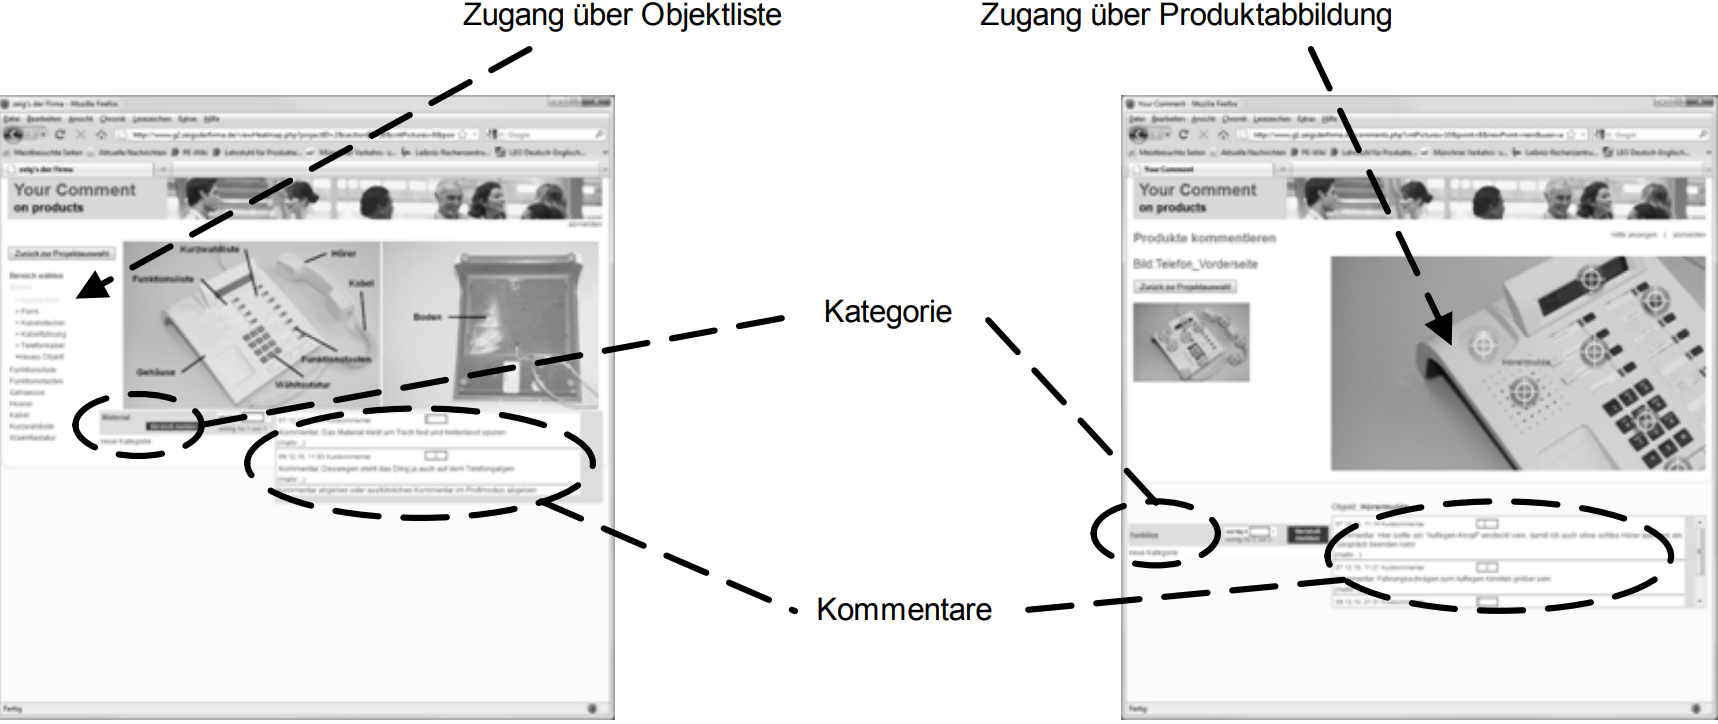
\includegraphics[width=0.8\textwidth]{resources/analyse/IPI_Vergleich_Listen_BildAnnotationeAnsicht.png}
	\caption{Online-Produktkommentierung über Listen- und Bildzugang. Quelle: \cite[S.~7]{Kirschner2011}}
	\label{img:ipi_list_image}
\end{figure}

\begin{figure}[H]
	\centering
	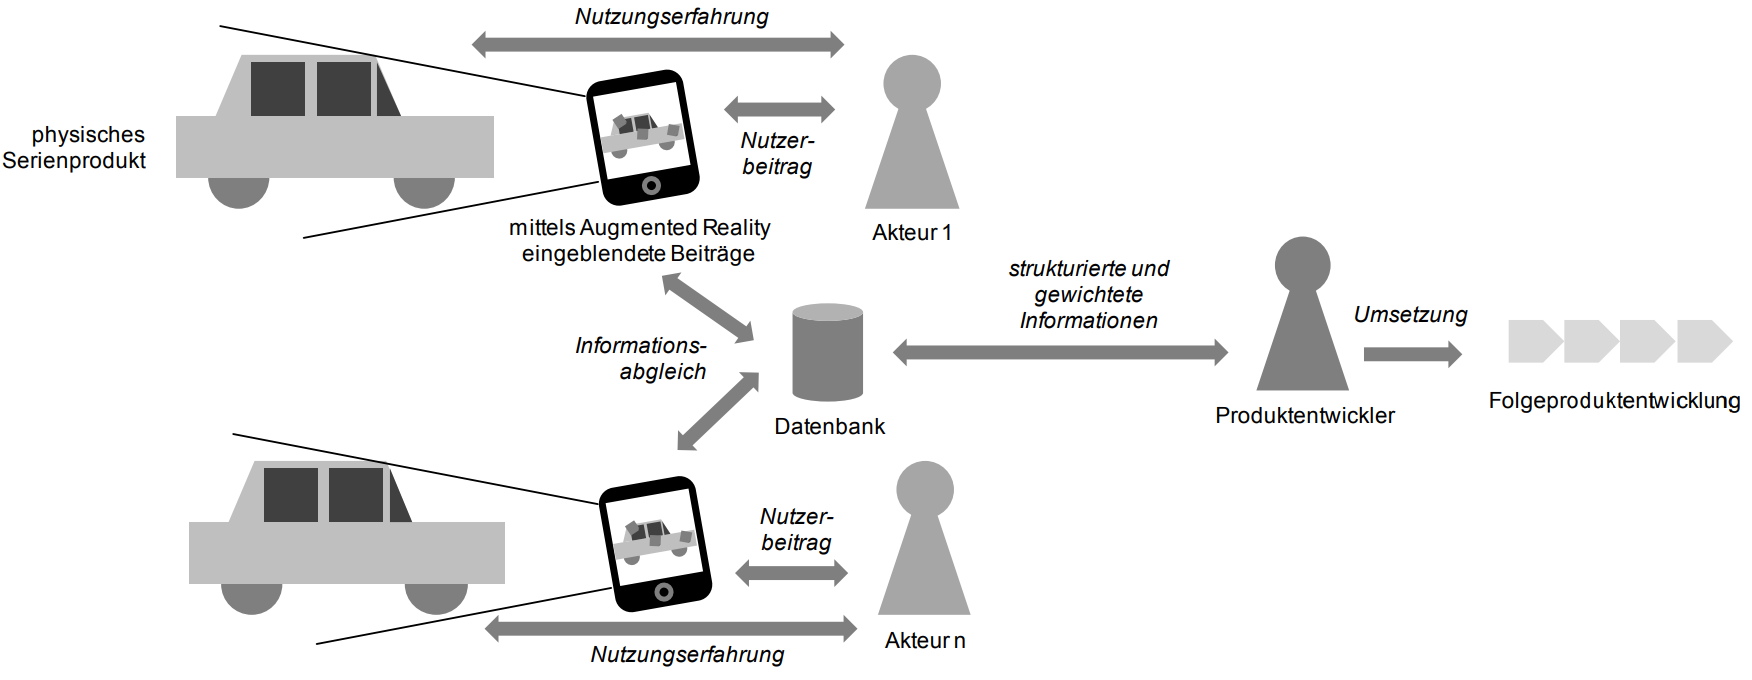
\includegraphics[width=0.8\textwidth]{resources/analyse/IPI_Objektzentriert.png}
	\caption{Informationsfluss  in der objektzentrierten IPI-Umsetzung. Quelle:\cite[S.~135]{Kirschner2012}}
	\label{img:objekt_centered_ipi}
\end{figure}


%kurz pysische 

%Bildzentriert. Vergleich mit Liste. Ergebnisse der Studie aus 2011

% Objektzentriert.

\section{Zusammenfassung}